\section{\system: A science gateway for bioinformatics extension to CSGrid}\label{sec:bioinfo}

This section presents the science gateway \system\footnote{\url{https://bioinfo.lncc.br}} which manages the execution of bioinformatics applications in HPC infrastructures. \system was built under the extension of the CSGrid\footnote{\url{https://jira.tecgraf.puc-rio.br/confluence/display/CN/CSGrid+Home}} middleware and coupled to the SDumont\footnote{\url{https://sdumont.lncc.br}} supercomputer. The \system gateway architecture is composed of four layers: \texttt{User Interface Layer}, \texttt{Management Layer}, \texttt{Data Layer}, and \texttt{Resource Layer}. Figure~\ref{fig:bioinfoportal} describes the conceptual view of the components of \system.

\underline{\textbf{User Interface Layer}} is the front-end which dynamically implements the interface of \system. Users interact with front-end to submit the executions of bioinformatics applications available in \system as software (\raxml) or workflows (\sci, \swift) and to return results sent by users’ e-mail. \underline{\textbf{Management Layer}} relies on the middleware CSGrid which allows the access of the submitted data and job management services. This layer provides the features for job/workflow scheduling, sharing files, restricting anonymous access, and tracking provenance data. \underline{\textbf{Resource Layer}} is composed of the computational resources (clusters and supercomputers) available by the SINAPAD centers distributed in several Brazilian research institutions. The computational resources host the bioinformatics software, libraries, SWfMS, and DBMS that are needed for executions. \underline{\textbf{Data Layer}} is formed by the databases and other repositories of \system and provides access to the input data and provenance data stored. This layer also authenticates the users using the repository Lightweight Directory Access Protocol (LDAP). The next sections discuss each component in details.

\begin{figure*}[!t]
\centering
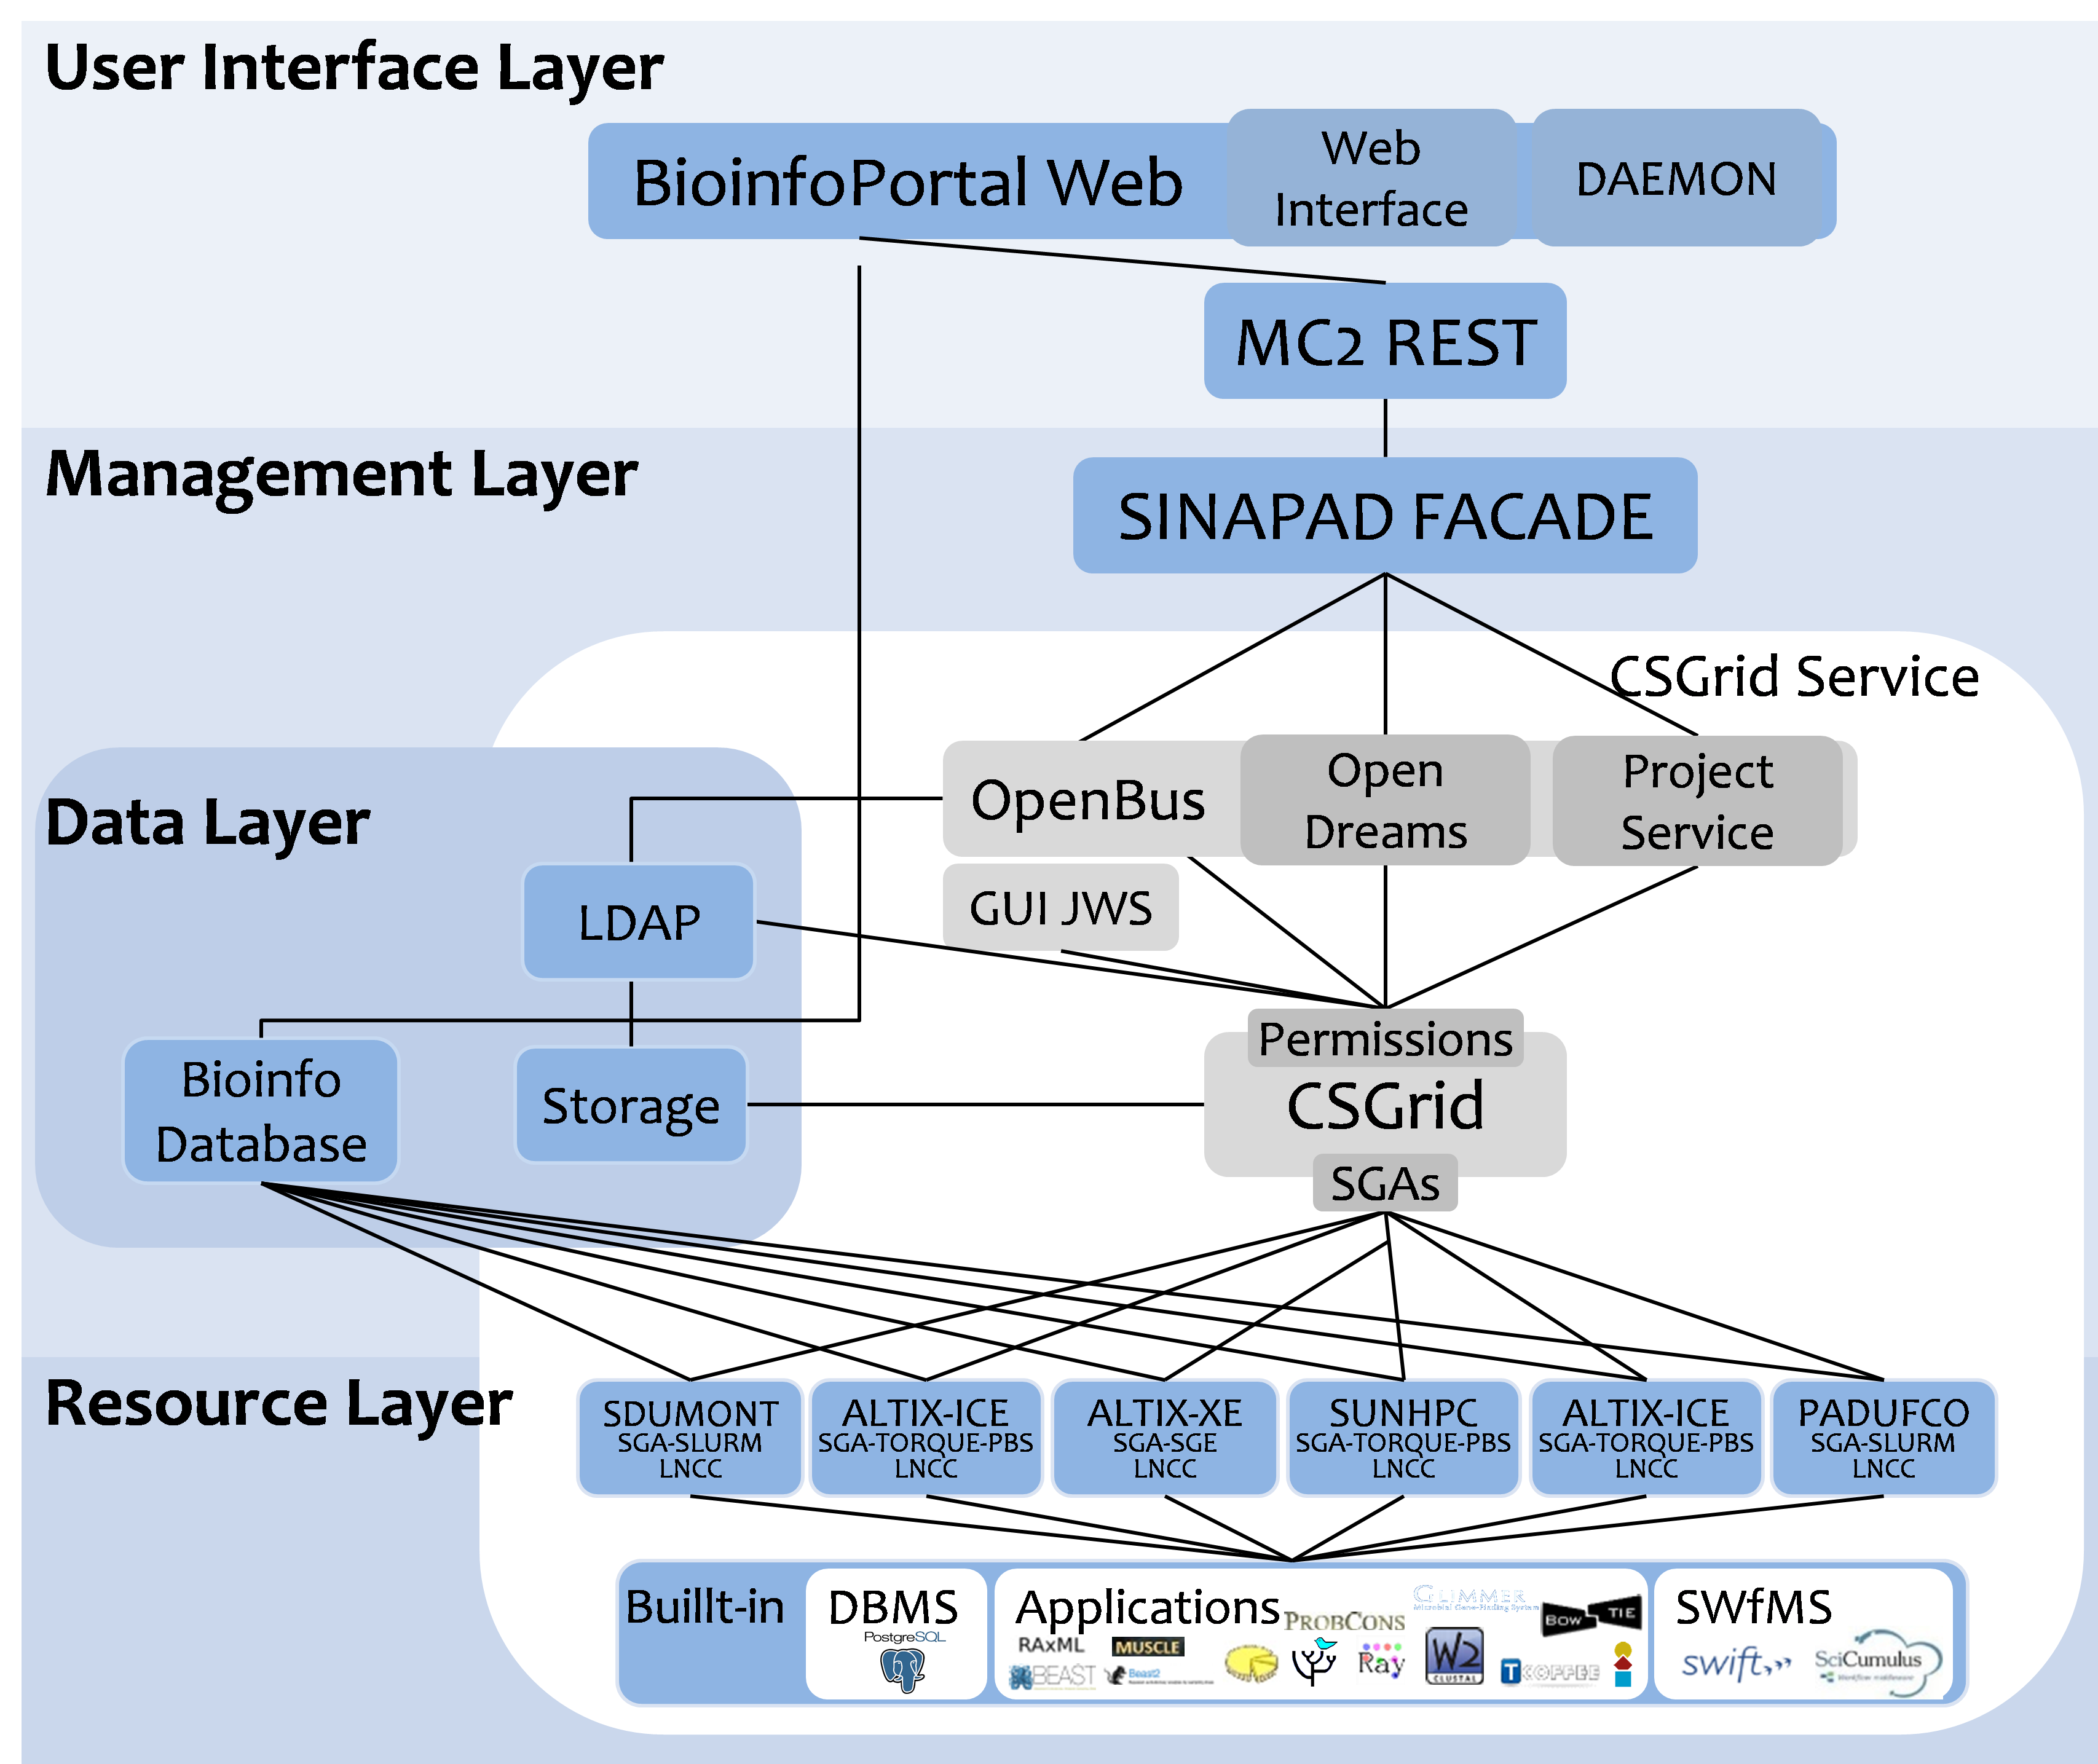
\includegraphics[width=0.75\textwidth]{imgs/bioinfoportal.png}
\vspace{-10px}
\caption{The \system architecture.}
\label{fig:bioinfoportal}
\end{figure*}

\subsection{The User Interface Layer (front-end)}

SINAPAD host several services and portals, as our science gateway \system and presents two main sub-layers: services and applications. \textbf{Services Sub-Layer} is composed of the MC2 services \cite{doi:10.1002/cpe.3258}, as the MC2 REST which dynamically interacts with other services provided by SINAPAD. \textbf{Applications Sub-Layer} is composed of web clients, such as our \system and presents two components: the Web interface and DAEMON. The Web Interface component is used as front-end by users and has an authentication strategy that categorizes the type of access (public or private) assigned to users, which need to be previously registered at SINAPAD through an electronic form. The public access (for guest users) is provided with no authentication, but the service administrator can restrict options for using the computing resources. The private access (for private users) is provided with authentication as the service administrator provides more flexibility or no restriction. The DAEMON component is a robust fault tolerance mechanism for dispatching and scheduling jobs/workflows. DAEMON is connected to the Data Layer at Bioinfo Database for providing an entry for accessing the provenance data information (records of executions or specific domain-data provenance of bioinformatics applications).
The actual version of \system has public access that allows users to choose software, parameters, and input data for submitting their jobs/workflows with no previous authentication.

\vspace{-5px}
\subsection{The Management Layer}

This layer is composed of three sub-layers: Facade, Bus Services, and CSGrid. \textbf{Facade Sub-Layer} enables the configuration for connecting the services (\system, SINAPAD’s services, HPC resources); searches the information needed for applications, clients, and users’ authentication; manages files; and submits/monitors jobs and resources. \textbf{Bus Services Sub-Layer} is implemented as a service-oriented software, called OpenBus, that allows for searching and publishing services by the client applications and for controlling the authentication/authorization of clients and services using internal governance management systems, digital certifications, and LDAP. \textbf{CSGrid Sub-Layer} is a client application of the OpenBus services (OpenDreams, ProjectService) that executes and manages data in the grid environment. CSGrid manages computational resources, clients, users, submissions, data, applications, and user databases (locally or LDAP) of \system at SINAPAD. CSGrid uses the Java-based graphical user interface (GUI) that allows SINAPAD to manage and implement internal applications. CSGrid presents three main conceptual definitions, more information please at XXX: Module, Concept, and Requisition. 

The \textbf{SGA Module} of CSGrid remotely manages the access of computational resources (Resource Layer). SGA is responsible for managing, submitting, scheduling, deleting, associating, and executing computational resources and jobs. SGA uses a pattern nomenclature, which is specific for each application executed in each cluster (sga-<sinapadName>-<schedulerType>-<resourceName>-<queueName>). SGA defines the best combination of settings (name, scheduler type, queue submission, parameters) to maintain the effective connectivity between SINAPAD’s computational resources.

The \textbf{Sandbox Concept} is a mechanism associated with the execution of the computational resources. It provides the availability, reliability, and security of the data using two stages: the stage-in allows users to submit the input data sets and the stage-out returns the results of the executions to the users of a Project at CSGrid. Figure~\ref{fig:raxmlalgorithm} presents the \textbf{Algorithm Concept} that is the structure at CSGrid where the configuration of the applications are available for users and administrators of \system. Algorithm describes the non-interactive applications (their information, input/output data, parameters) that are dispatched directly by the clients of CSGrid. Algorithm provides the information of applications – name, version, and features of installation/compilation in computational resources and configures the client interface. For instance, as the application Align-m was installed in the clusters sun.hpc, altix-xe, ice, sdumont; then the Algorithm Align-m can be created at CSGrid and consequently. This way, all interfaces of SINAPAD as our \system (or others services) are able to access the Algorithm Align-m, to call it, and execute the application Align-m in the clusters sun.hpc, altix-xe, ice, or sdumont.

The \textbf{Requisitions} of SINAPAD allow selecting the computational resources that are available and free at the moment. There are two modes of Requisitions: by users who need to choose the parameters, configurations, and clusters or by schedulers which automatically decide which resource is eligible for submissions. The metric used for schedulers is the number of free Central Processing Units (CPUs) in each cluster. Other metrics as the amount of free memory, disk space, network latency, or job submissions can be included by implementing new plugins. The configuration of the actual version of \system uses public access (no user authentication) with automatic submissions using the mode of the automatic mode by schedulers, but it can be also re-configured.

\vspace{-5px}
\subsection{The Data Layer}

This layer presents four sub-layers the LDAP, Storage, Bioinfo Database, and Scientific Workflow Management Systems (SWfMS) Databases. The \textbf{LDAP Sub-Layer} manages the authentication of users for the portals of SINAPAD. The \textbf{Storage Sub-Layer} stores the information of the user data, application credentials, algorithm configurations, user/application permissions, and execution history proceeding of the application portals and CSGrid. The \textbf{Bioinfo Database Sub-Layer} stores the information (job monitoring, tasks executions, provenance data) proceeding of the applications executed in SINAPAD resources. The The \textbf{SWfMS Database Sub-Layer} includes the provenance databases of the SWfMS SciCumulus \cite{5557969} and Swift \cite{article}. 

The management of the provenance data \cite{e2df054d304d4601be3c733a9d73ff5d} records the history of executions and supports the analysis of scientific experiments. The SciCumulus database follows the data model PROV-Df and W3C PROV and uses the PostgreSQL Relational Database Management System (RDBMS) to manage at runtime the provenance data information consisting of the performance of executions, structure of workflows, and domain-data. Swift is a script programming language for scientific workflows. It uses the server-less SQLite relational database for storing the provenance data. 
The decision-making or fault-tolerance predictions are possible by extracting the provenance information from the databases of Bioinfo and SWfMS and by coupling data mining and machine learning techniques. For instance, provenance information about which tasks are running in which clusters or if the capacity of processing time and memory is enough could be used to predict/prevent errors of executions. Those errors could affect the functionality of services and portals of SINAPAD (including \system) and must be detected. 

\vspace{-5px}
\subsection{The Resource Layer}

The computational resources of SINAPAD are formed by clusters, grids, and public/private clouds. A heterogeneous HPC cluster environment can contain processors and devices with different bandwidth and computational capabilities. Due to that reason, the installation or compilation of the applications and dependencies is made manually by developers/clients, following some requirements: (i) using parameters that optimize the compilation and installation of applications, libraries, and dependencies; (ii) using, as possible, mechanisms and technologies to distribute and parallelize tasks, \textit{i.e.} graphics processor unit (GPU), message passing interface (MPI), or threads; (iii) using mechanisms for optimizing the submissions of schedulers Torque/PBS, SGE, SLURM, Load Leveler; (iv) optimizing the use/configuration of parameters for SWfMS; and (v) coupling to Data Layer, resources as DBMS to register the provenance.

The Resource Layer presents two sub-layers. The \textbf{Applications Sub-Layer} formed by 35 software installed, compiled, and deploted in each cluster of SINAPAD. The \textbf{SWfMS Sub-Layer} formed by the SWfMS SciCumulus \cite{5557969} and Swift \cite{WILDE2011633}, which greatly reducing the complexity of managing experiments by providing features for scalable execution, scalable data management, fault-tolerance, and provenance data tracking \cite{mattoso2010}. The integration of the SWfMS to middleware CSGrid, and the computational resources of SINAPAD require steps, detailed as follows. For SciCumulus, we implemented: (i) a network proxy that allows accessing to the SciCumulus provenance database; (ii) modification of the scripts of configuration (XML) and execution of applications (bash scripts) of SciCumulus, (iii) new bash scripts for mining labels (“tags” in the XML scripts of SciCumulus); and (iv) a connection between the databases of SWfMS and Bioinfo sub-layers. For Swift, we implemented bash scripts to (i) configure Swift at the HPC resources of SINAPAD; (ii) connect the database SQLite to CSGrid and SINAPAD; and (iii) configure the environment to manage execution jobs from a submission node to the clusters.

\vspace{-10px}

